\section{Introduction}

In the last years, recurrent neural networks \cite{Elman:1990}, in
particular in their long-short-term-memory (LSTM) variant
\cite{Hochreiter:Schmidhuber:1997}, have been successfully applied to
a variety of challenging NLP tasks. This has spurred interest in
whether these generic sequence-processing devices are inducing
structural properties of language from their training data, or whether
their success can be explained away by opportunistic
heuristics. Starting with the seminal work by
\newcite{Linzen:etal:2016}, long-distance number agreement (``the
\textbf{boy} behind the trees \textbf{greets}\ldots'') has played a
central role in this debate. After mixed initial results by Linzen and
colleagues and \newcite{Bernardy:Lappin:2017},
\newcite{Gulordava:etal:2018} and \newcite{Kuncoro:etal:2018a} have
robustly established that LSTMs trained with the language modeling
objective on raw data predict the correct agreement with human-like
performance. While Gulordava and colleagues provided some evidence
that the LSTMs are relying on genuine syntactic generalizations,
\newcite{Kuncoro:etal:2018b} and \newcite{Linzen:Leonard:2018}
suggested that the LSTM achievements can, at least in part, be
accounted by superficial heuristics.

Until now, this debate has been based on ``behavioural'' evidence: The
LSTM is treated as a black box, and its capacities are indirectly
inferred by performance on linguistic tasks. This paper takes a
complementary ``neuroscientific'' approach. We thoroughly investigated
the inner dynamics of an LSTM performing the number agreement task,
coming closer to a mechanistic understanding of how it accomplishes
the task.

We found that the LSTM specialized very few ``grandma'' cells
\cite{Bowers:2009} to carry number features from a sentence subject to
the verb across other material. Interestingly, the LSTM also possesses
a more distributed mechanism to predict number when subject and verb
are close, with the number cells only playing a crucial role in more
difficult long-distance cases. Crucially, we independently identified
a set of cells that track syntactic structure, and found that one of
these syntax-aware cells has strong efferent connections to the
long-distance number cells, suggesting that the network relies on
genuine syntactic information to determine agreement.

Our analysis thus provides more direct evidence for the claim that
LSTMs trained on unannotated corpus data with the unsupervised
language modeling task, despite lacking significant linguistic priors,
are developing structure-dependent linguistic mechanisms. In turn,
this suggests that raw linguistic input and generic memory mechanisms
such as those implemented in the LSTM, might suffice to trigger the
learning of non-trivial grammatical rules.

\textbf{The following fragments should probably go in the
  conclusion. I'm not sure of where the bit on the plural/singular
  asymmetry should go (I don't think we should emphasize the
  ``behavioural'' part of it, as that's tangential to the story in
  this paper.}

More generally, we provided the most detailed analysis of the inner
dynamics of an LSTM performing a linguistic task we are aware of. We
think that similar studies should complement currently popular
black-box tests, to achieve a true understanding of language
processing in neural networks. \textbf{Here, we might want to mention
  the need for future work on relative clauses, as well as on other
  models, such as transformers.0}

\ldots From a more cognitive perspective, we hope our granular
understanding of how LSTMs perform number agreement will inform work
on computational modeling of neural sentence processing data, as we
conjecture a similar interaction between syntactic and
feature-carrying units might be implemented in the human
brain. Intriguingly, we observed differential handling of singular and
plural information, with the latter being more reliably processed,
resulting in more robust plural agreement. As a similar asymmetry has
also been observed in humans (\textbf{REFS}), one exciting avenue for
future work might consist in looking for different singular/plural
processing networks in the human brain.


\begin{figure}
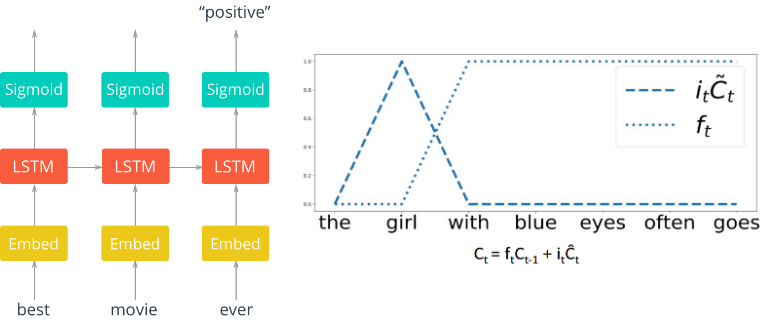
\includegraphics[width=\linewidth]{Figures/Figure1_intro.png}
\caption{Caption.}
\end{figure}
